\section{Approach}
\label{sec:approach}

The DMAS solution we developped defines two agents, \emph{Package Agents} and
\emph{Truck Agents}. All Package Agents have a corresponding package and are
located on the pickup location of that package. Truck Agents control a
corresponding truck and move along with the truck. Both agents also own a
\emph{pheromon table}. These tables can hold multiple paths (list of Package
Agents in a certain order) and a corresponding pheromon (heuristic value).

\npar Package Agents and Truck Agents communicate with each other by sending
ants. These are a sort of smart messages.

\npar There is also a \emph{"forwarder"} placed in each delivery location of a
package. These \emph{"forwarders"} will send all received ants to the Package
Agent corresponding with the package for the local delivery location. Because of
their limited intelligence, forwarders are not considered to be agents.

\npar Like most DMAS based on ACO, three type of ants will be used. They will be
used in the following way:

\begin{description}
	\item[Feasability Ants] These ants will be periodically broadcasted
	over a certain radius from the Package Agents to the forwarders (delivery
	locations). Their main purpose is to inform other Package Agents wich Package
	Agents are in a certain radius near their delivery location.

	\item[Exploration Ants] These ants will be sent from the Truck Agents
	to discover and evaluate a path of Package Agents. They will update the
	pheromons table in the Package Agents during their return over the discovered
	path.
	
	\item[Intention Ants] These ants will be sent from the Truck Agents
	over the path of Package Agents that they are planning to follow. These ants
	will decrease the pheromon values for that path in the visited Package Agents
	in order to discourage other agents to follow this path.
\end{description}

\npar How agents find an optimal path by using the pheromones and communication
over ants is further explained in the following scenarios.

\subsection*{Scenario I: Broadcasting of Feasibility Ants}
\label{subsec:scenario1}

When Package Agent A (depicted as a brown box 'A' in Figure \ref{Fig:scenario1})
is added to the simulation it will broadcast a Feasibility Ant with origin
\emph{"A"} in a certain radius to all delivery locations (forwarders, depicted
as a yellow flags in Figure \ref{Fig:scenario1}). Forwarders C' and B' receive
the feasibility ant and send it to their corresponding Package Agents C and B.
These Package Agents now know that after their packages are delivered, package A
is near. After C and B have added path \emph{"A"} to their tables with a default
pheromon value, they will change the origin of the Feasibility Ant to "CA" and
"BA" respectively and broadcast it again. This time, on

This process goes on until the max number of hops (= number of times broadcasts

\npar The max number of hops for Feasibility ants is in our application 1, i.e. only


\begin{figure}[!h]
        \vspace{0.5pt}
        \begin{center}
       			\setlength\fboxsep{0.5pt}
				\setlength\fboxrule{0.5pt}
                \fbox{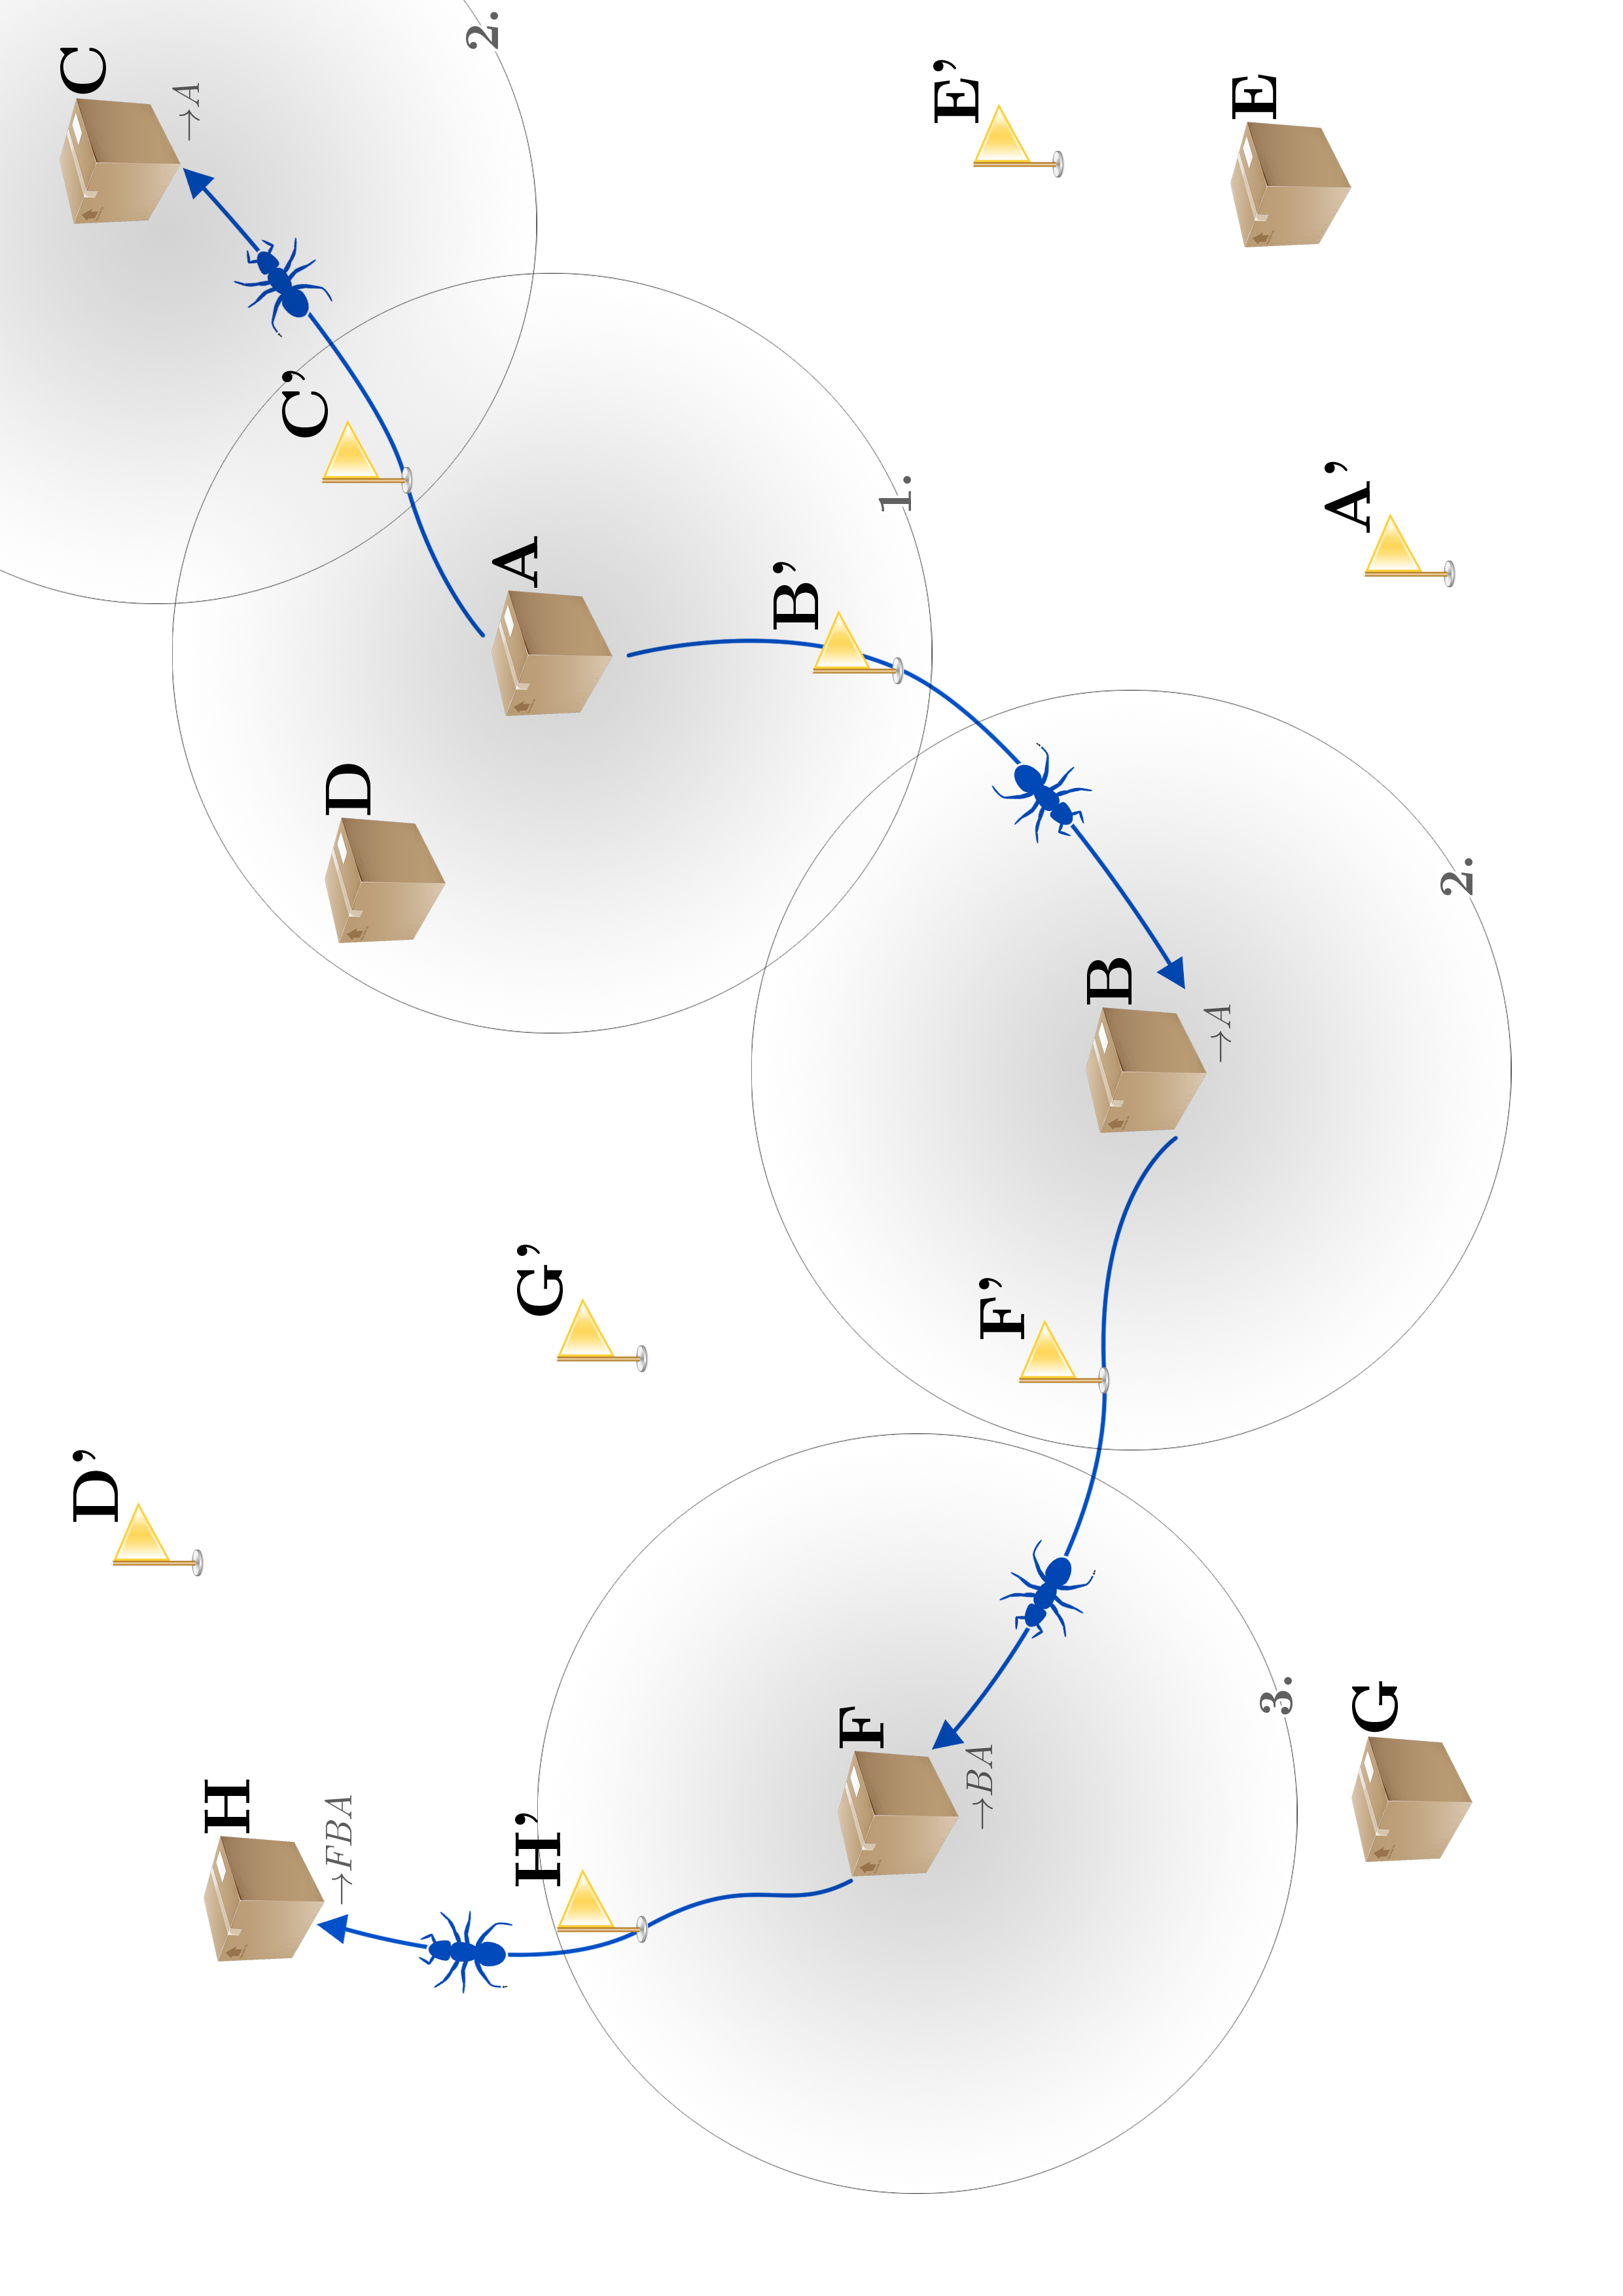
\includegraphics[width = 0.90\textwidth]{./figs/feasibility.png}}
		\end{center}
		\caption{Example Scenario I (\ref{subsec:scenario1})}
		\label{Fig:scenario1}
        \vspace{0.5pt}
\end{figure}

\begin{figure}[!h]
        \vspace{0.5pt}
        \begin{center}
       			\setlength\fboxsep{0.5pt}
				\setlength\fboxrule{0.5pt}
                \fbox{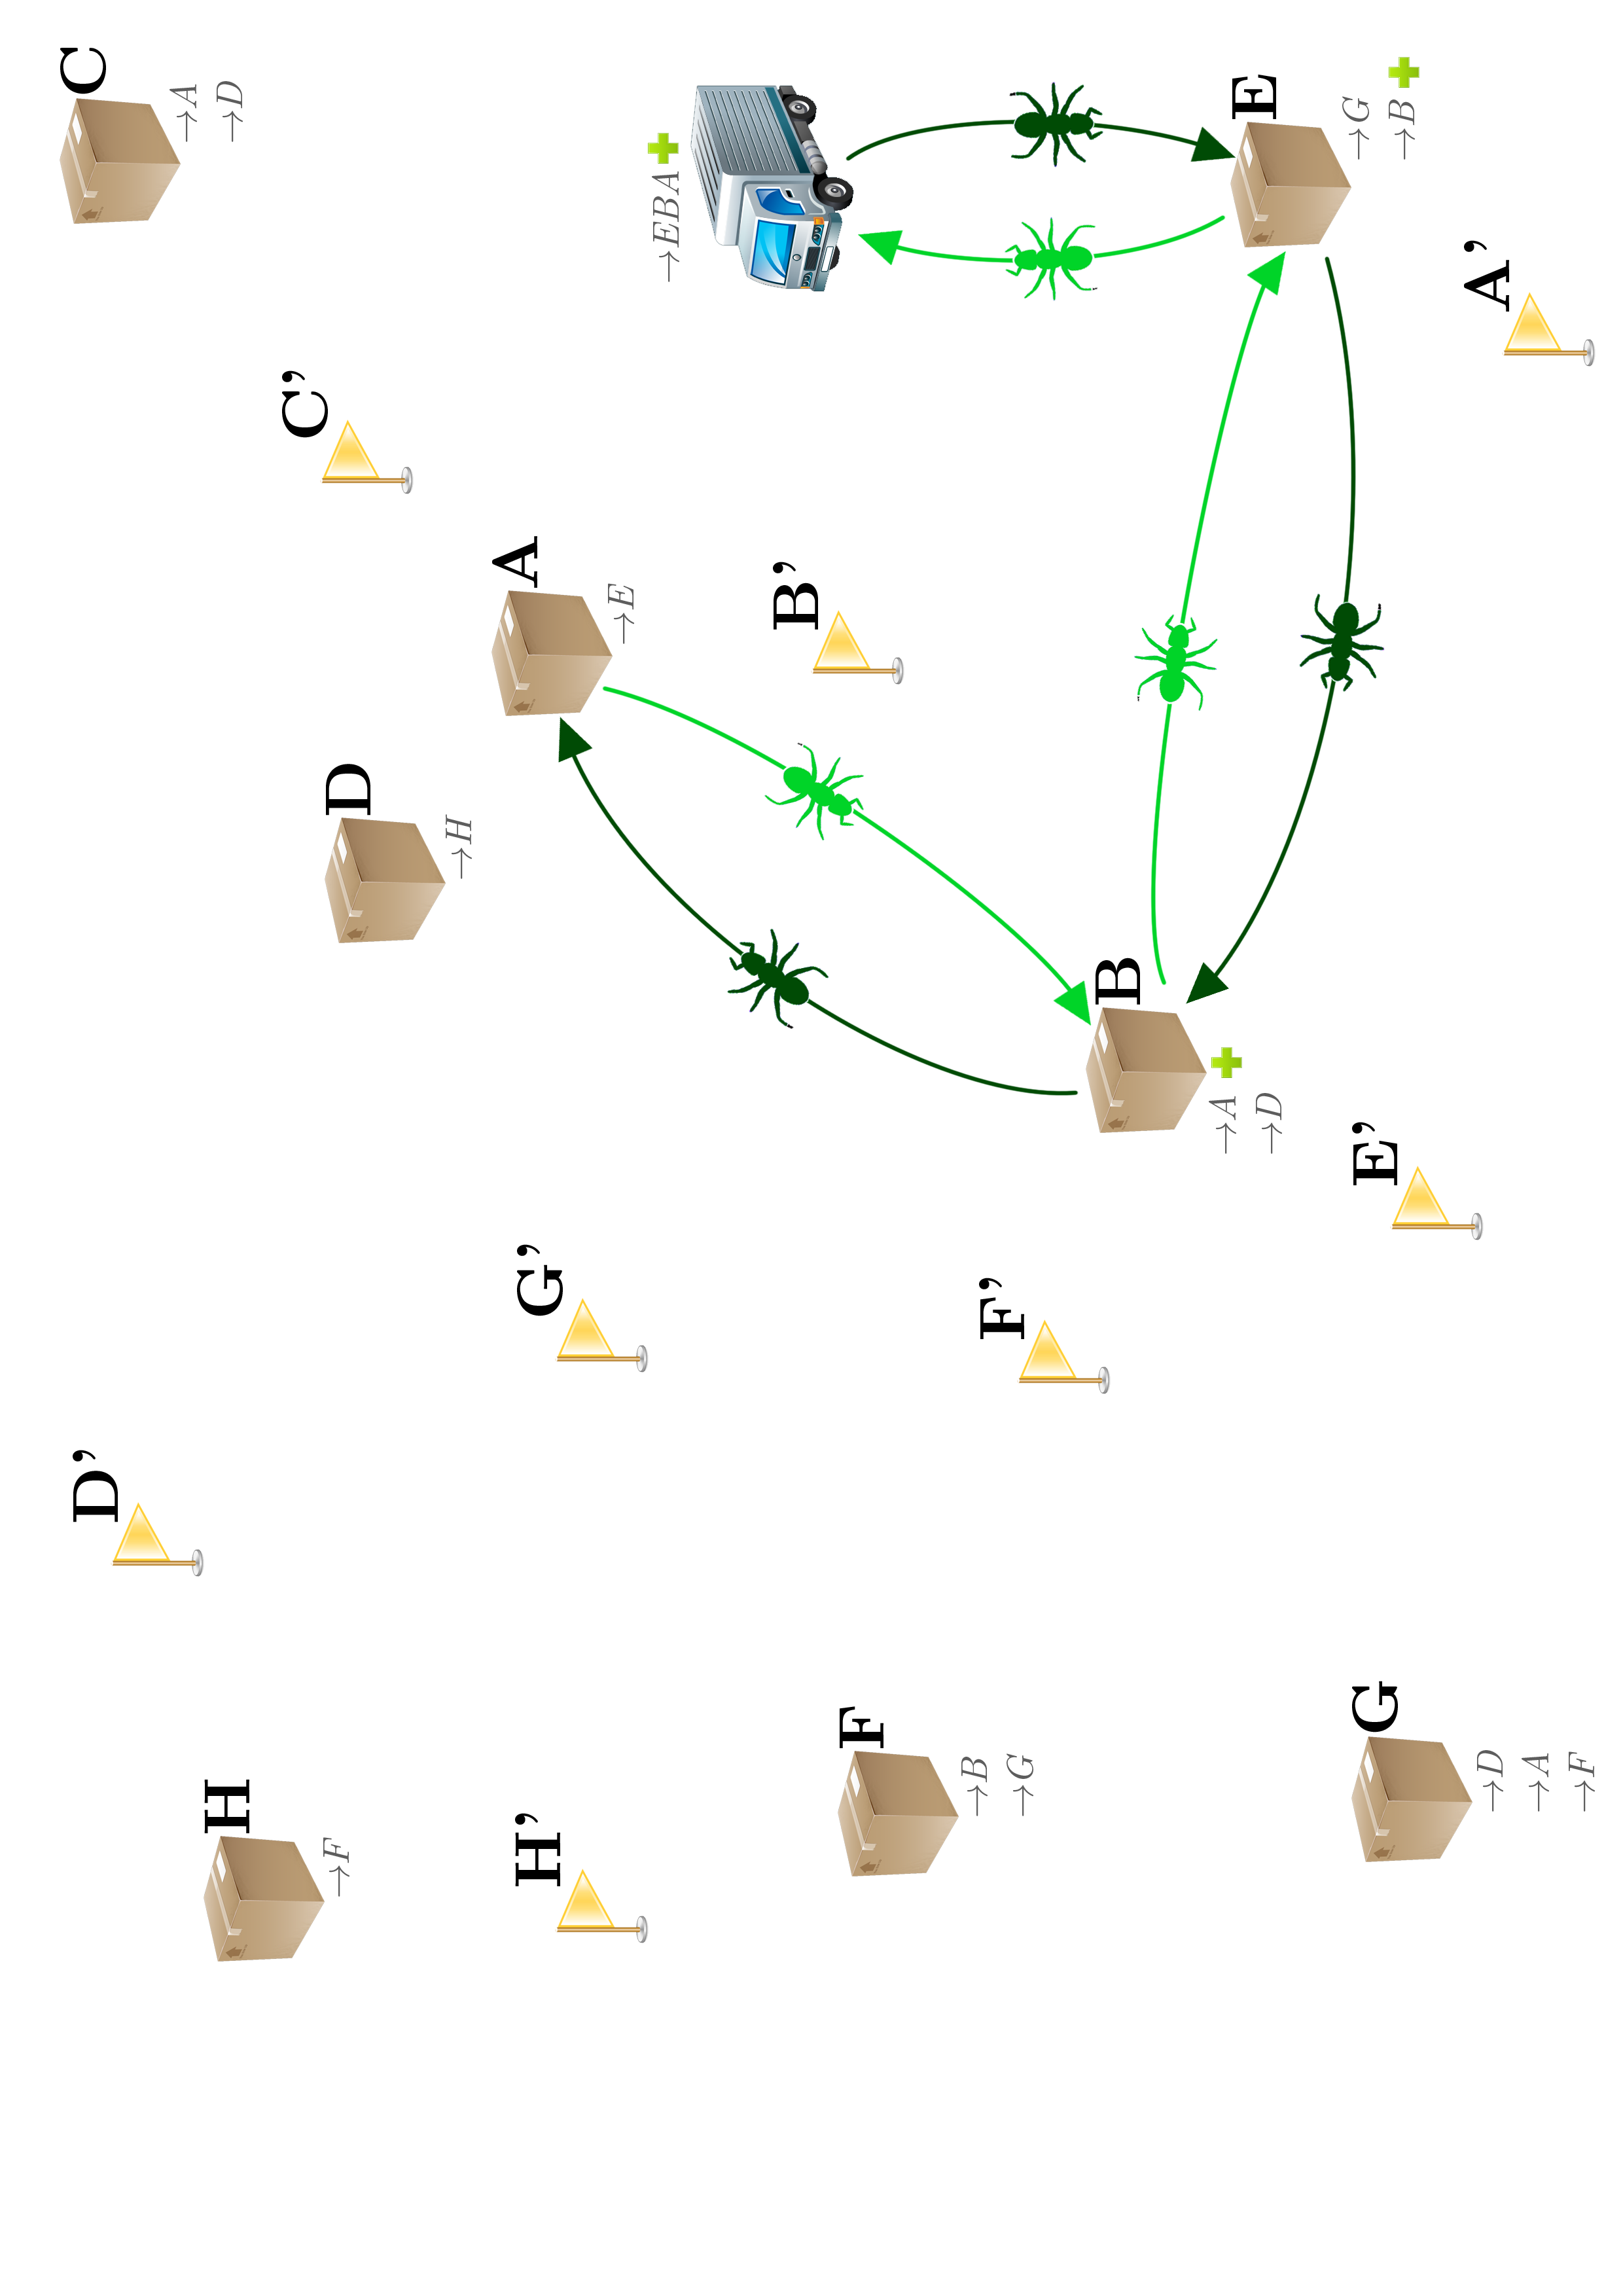
\includegraphics[width = 0.90\textwidth]{./figs/exploration.png}}
		\end{center}
		\caption{Exploration Ants (example scenario 2)}
		\label{Fig:Radios}
        \vspace{0.5pt}
\end{figure}

\begin{figure}[!h]
        \vspace{0.5pt}
        \begin{center}
       			\setlength\fboxsep{0.5pt}
				\setlength\fboxrule{0.5pt}
                \fbox{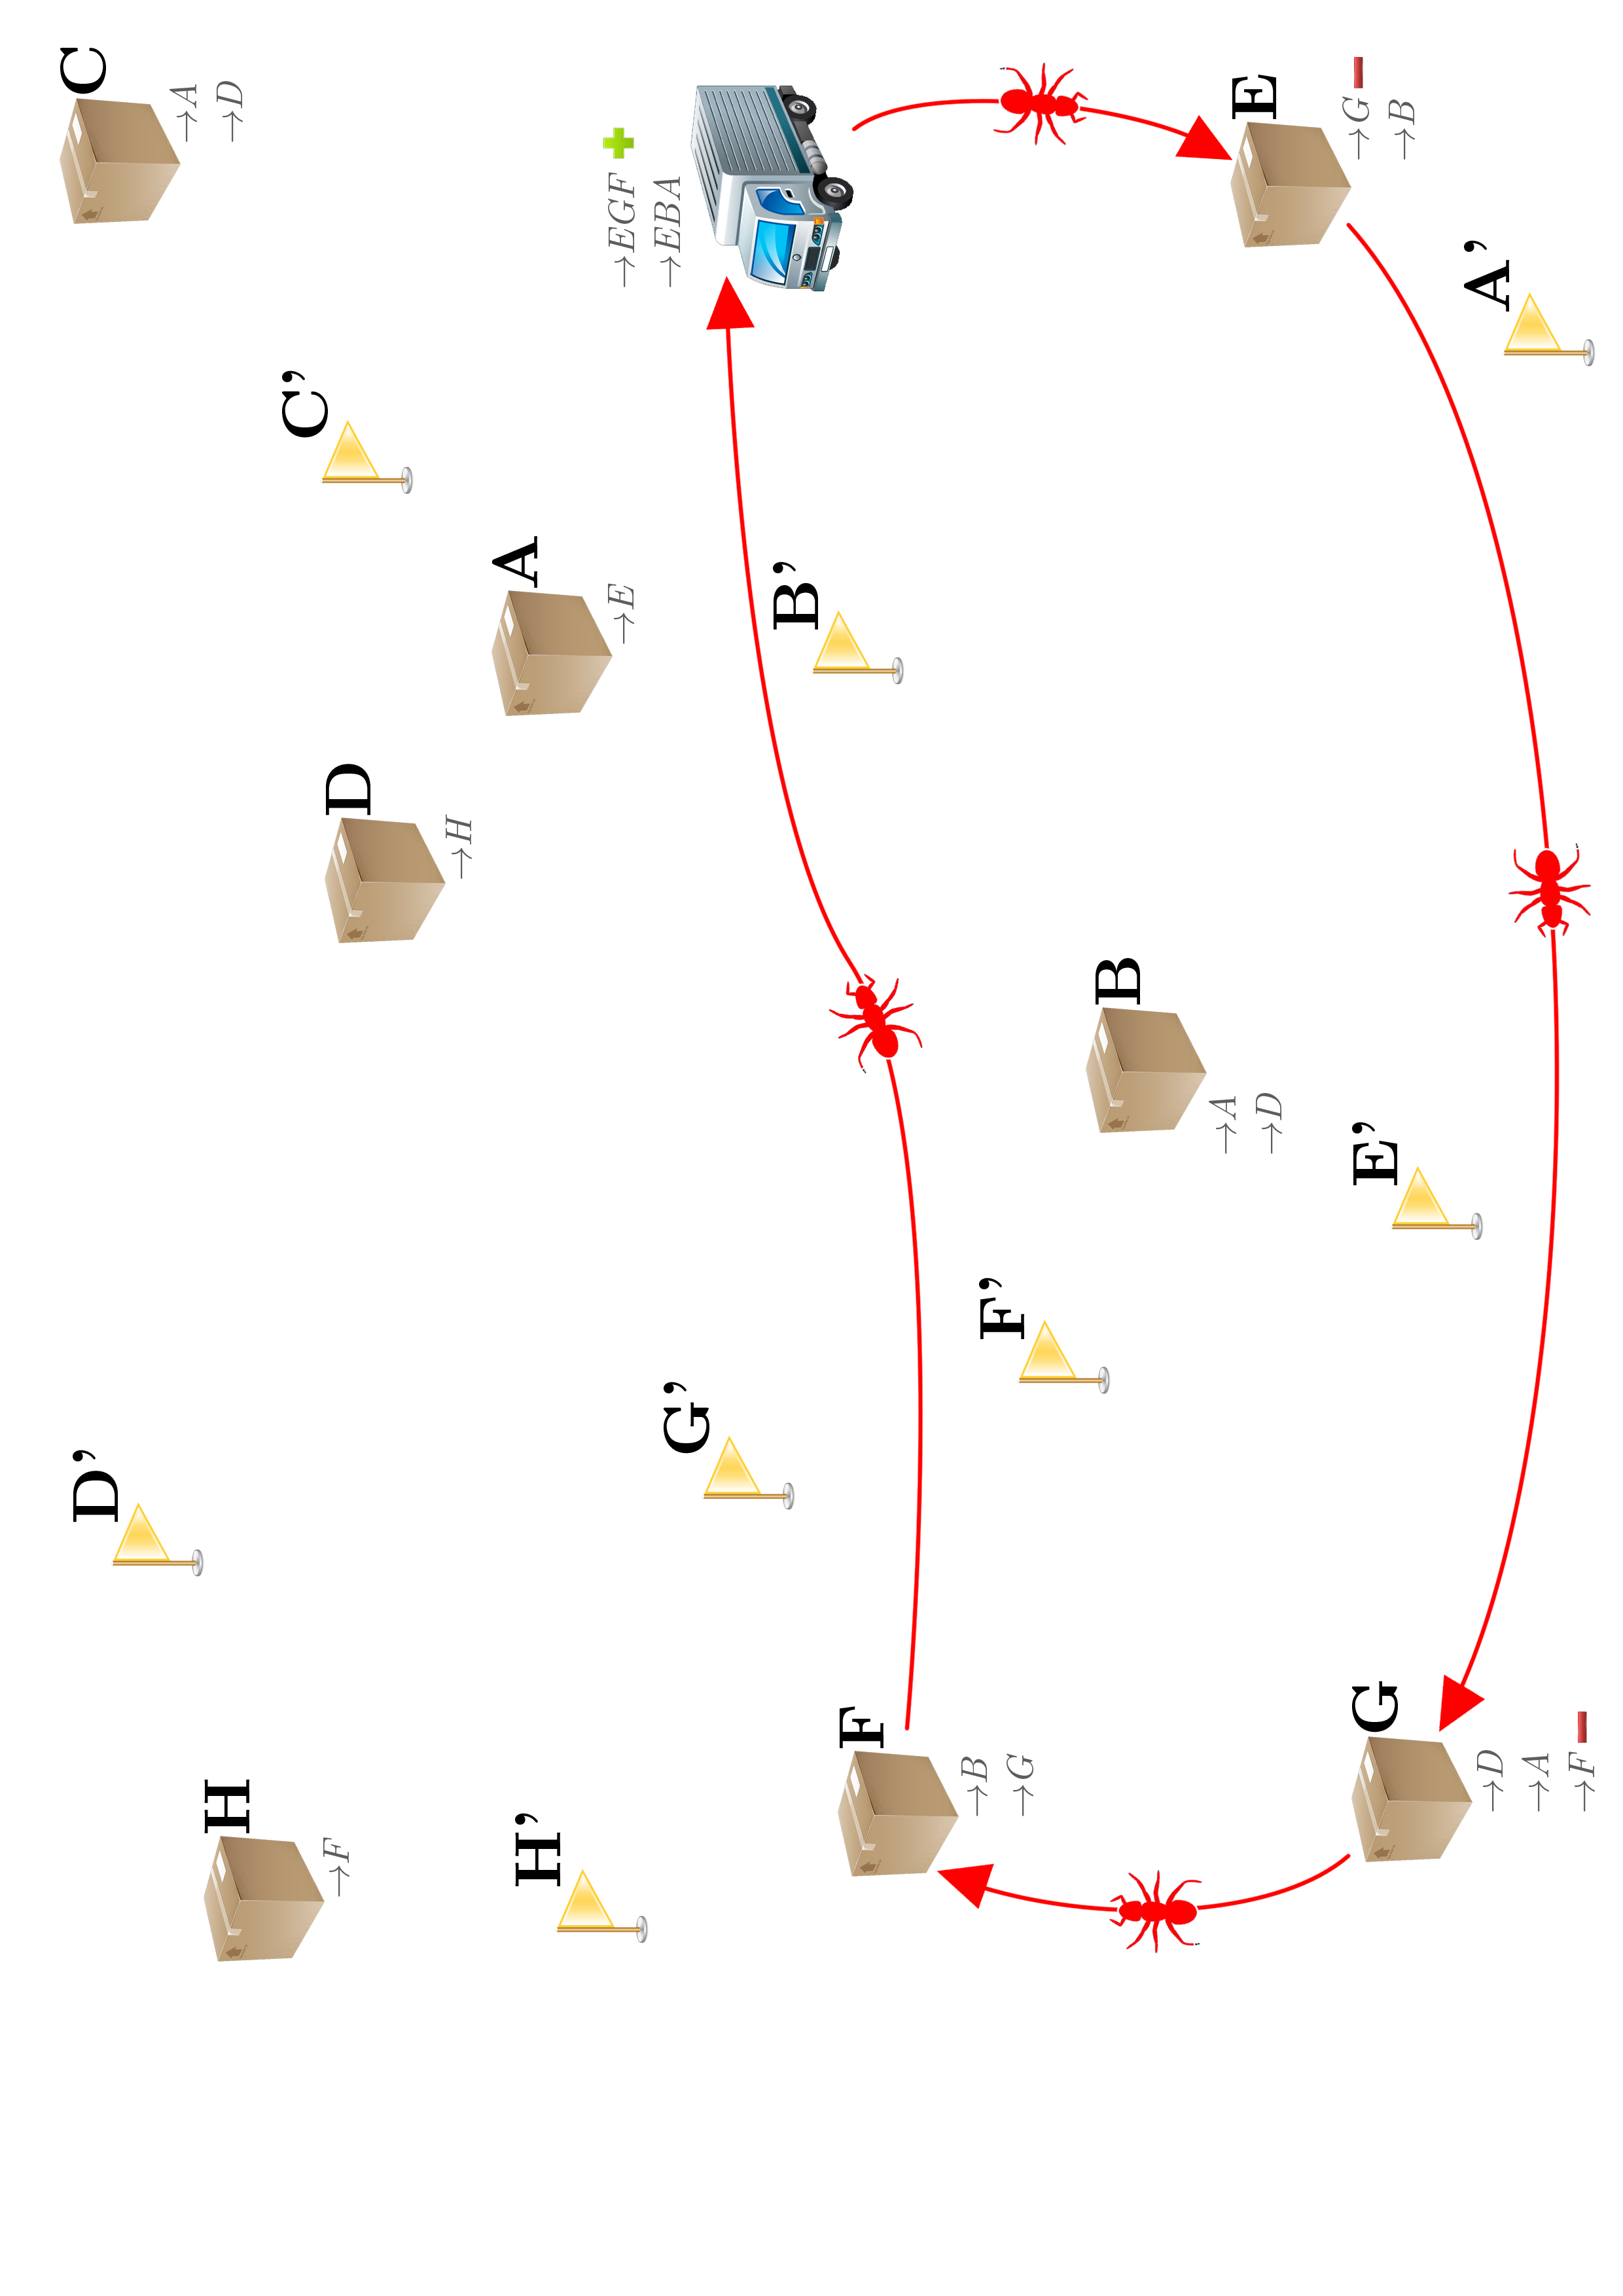
\includegraphics[width = 0.90\textwidth]{./figs/intention.png}}
		\end{center}
		\caption{Intention Ants (example scenario 3)}
		\label{Fig:Radios}
        \vspace{0.5pt}
\end{figure}
